\documentclass[main.tex]{subfiles}

\clearpage
% Intro
\section{Purely hyperbolic model problem}
One dimensional unsteady advection problem is defined as follows:
\begin{alignat}{3}
  & \partial_t u(x,t) + a \partial_x u(x,t) = 0, \qquad && -1 \leq x \leq 1, && t > 0, \\
  & u(-1,t) = u(1,t), && && t > 0, \\ 
  & u(x,0) = \eta(x), && -1 \leq x \leq 1.
\end{alignat}
the constant term $a$ is called advection speed. Given the periodic boundary conditions and the constant advection speed solution arises in the form 
\begin{equation}
  u(x,t) = f(x - a t)   
\end{equation}
(see the assignment handout). In this section $f$ is assumed to be $f(x) = \sin(2 \pi x)$ and $a = 0.5$. One could then write the solution as $u(x,t) = \sin(2 \pi x - \pi t)$.

% 2.1
\subsection{Stability of the FTBS scheme}
The numerical scheme that will be used is called \textit{Upwind}. It approximates the spatial derivative using only previously obtained information. Refering to LeVeque, the upwind method is used for positive values of $a$ in the advection problem, i.e. the solution travels from left to right. If $a$ was negative the downwind scheme would have been used.
\subsubsection*{Definition}
The upwind scheme has non-symmetric approximations to derivatives (one-sided approximations, backwards space). Taking the forward time differencing the method is defined as:
\begin{equation}
    U^{n+1}_j = U^n_j - \underbrace{a \frac{\Delta t}{\Delta x}}_{\nu}(U^n_j - U^n_{j-1})
\end{equation}
where $\Delta t$ and $\Delta x$ are the time and space steps respectively, and $\nu$ is the Courant number.
\subsubsection*{Stability -- von Neumann analysis}
In order to perform the analysis the term $U^n_j$ is rewritten as $g(\xi)^n e^{i \xi j h}$ (see LV 10.5), where $i$ is the imaginary number, $h$ is the space step (sometimes referred to as $\Delta x$) and for convenience $\theta = \xi \Delta x$. The wave number $\xi$ is defined as $\frac{2 \pi}{L}$ and $g(\xi)$ is called the amplification factor. Substituting into the upwind method definition:
\begin{equation}
\begin{aligned}
    g(\xi)^{n+1} e^{i \xi j h} &= g(\xi)^{n} e^{i \xi j h} - \nu \left(g(\xi)^{n} e^{i \xi j h} - g(\xi)^{n} e^{i \xi (j-1) h}\right) \\
    g(\xi)^{n+1} &= g(\xi)^{n} - \nu g(\xi)^n \left( 1 - e^{-i \xi h} \right) \\
    g(\xi) &= 1 - \nu (1 - e^{-i \theta}) \\
    g(\xi) &= 1 - \nu + \nu e^{-i \theta} \\
    g(\xi) &= 1 - \nu + \nu \left(\cos(\theta) - i \sin(\theta)\right) 
\end{aligned}\label{ex2:eq:neumann}
\end{equation}
Requiring the amplification factor to be bound by 1 in magnitude produces the stability bounds for the method (LV 10.5). In this case it is clear that $g(\xi)$ is a circle centered at $1 - \nu$ with radius equal to the Courant number. To satisfy the aforementioned bounds $g(\xi)$ needs to be contained in a unit circle in the complex plane, which is only possible when the Courant number is between 0 and 1 (inclusive).
\begin{figure}[h]
    \centering
    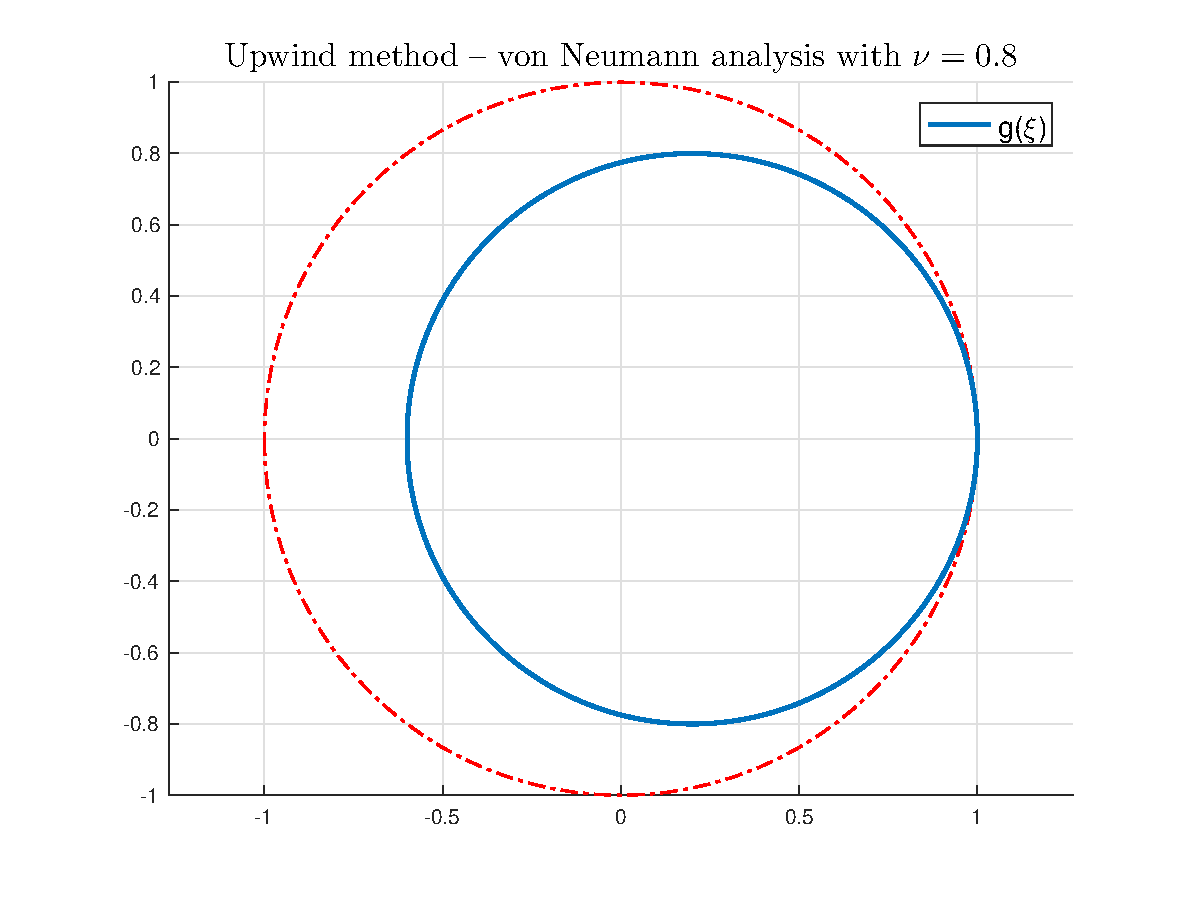
\includegraphics[height=3in]{../Figures/ex2_1_stability}
    \caption{$g(\xi)$ evaluated on the complex plane for $\nu = 0.8$ and $\Delta x = \frac{1}{100}$. The red dashed circle indicates the unit circle and the blue $g(\xi)$ is clearly within bounds, which confirms results of the previous analysis.}
\end{figure}

% 2.2
\subsection{Matlab implementation of FTBS and convergence}
The Matlab implementation is rather straight forward and shown in the listing below with comments provided in the code.

The choice of the input arguments can vary as there are multiple ways of calculating the parameters. For example it would be trivial to change the method signature to accept the Courant number $\nu$ instead of $\Delta x$.
\begin{lstlisting}[language=Matlab]
function [ U, Utrue ] = upwind( uFn, a, dx, dt, xmin, xmax, tmax )
% uFn - used to calculate u(x,0)
% a, dx, dt - user passed, used calculate Courant number (method signitature can be changed to pass in Cr directly if needed)
% xmin, xmax - spatial domain
% tmax - run until this time

t = 0;
steps = tmax/dt;
cr = (a*dt/dx);

x = xmin:dx:xmax;
N = length(x) - 1;
j = 2:N+1;

u0 = uFn(x,0);
u = u0;
unext = u0;

U = zeros(steps+1, N+1);
U(1,:) = u0;

Utrue = U; % this will be later overwritten, add only u0 for now

for n=2:steps+1
    % Keep track of time for calculating the true solution
    t = t+dt; 
    % Next u
    unext(j) = u(j) - cr*(u(j) - u(j-1));
    unext(1) = u(1) - cr*(u(1) - u(N)); % account for periodic BCs
    % Update the iterate and save
    u = unext;
    U(n,:) = unext;    
    % Calculate the true u
    Utrue(n,:) = uFn(x,t);
end

end
\end{lstlisting}%end code
\subsubsection*{Convergence of the solver}
Results from the theory show the convergence rate will be $\mathcal{O}(\Delta t + \Delta x)$ because of the spatial approximation combined with the Euler's method (forward in time) as shown in slide 20 from Lecture 22. Let's try to verify that.
\begin{figure}[h]
    \centering
    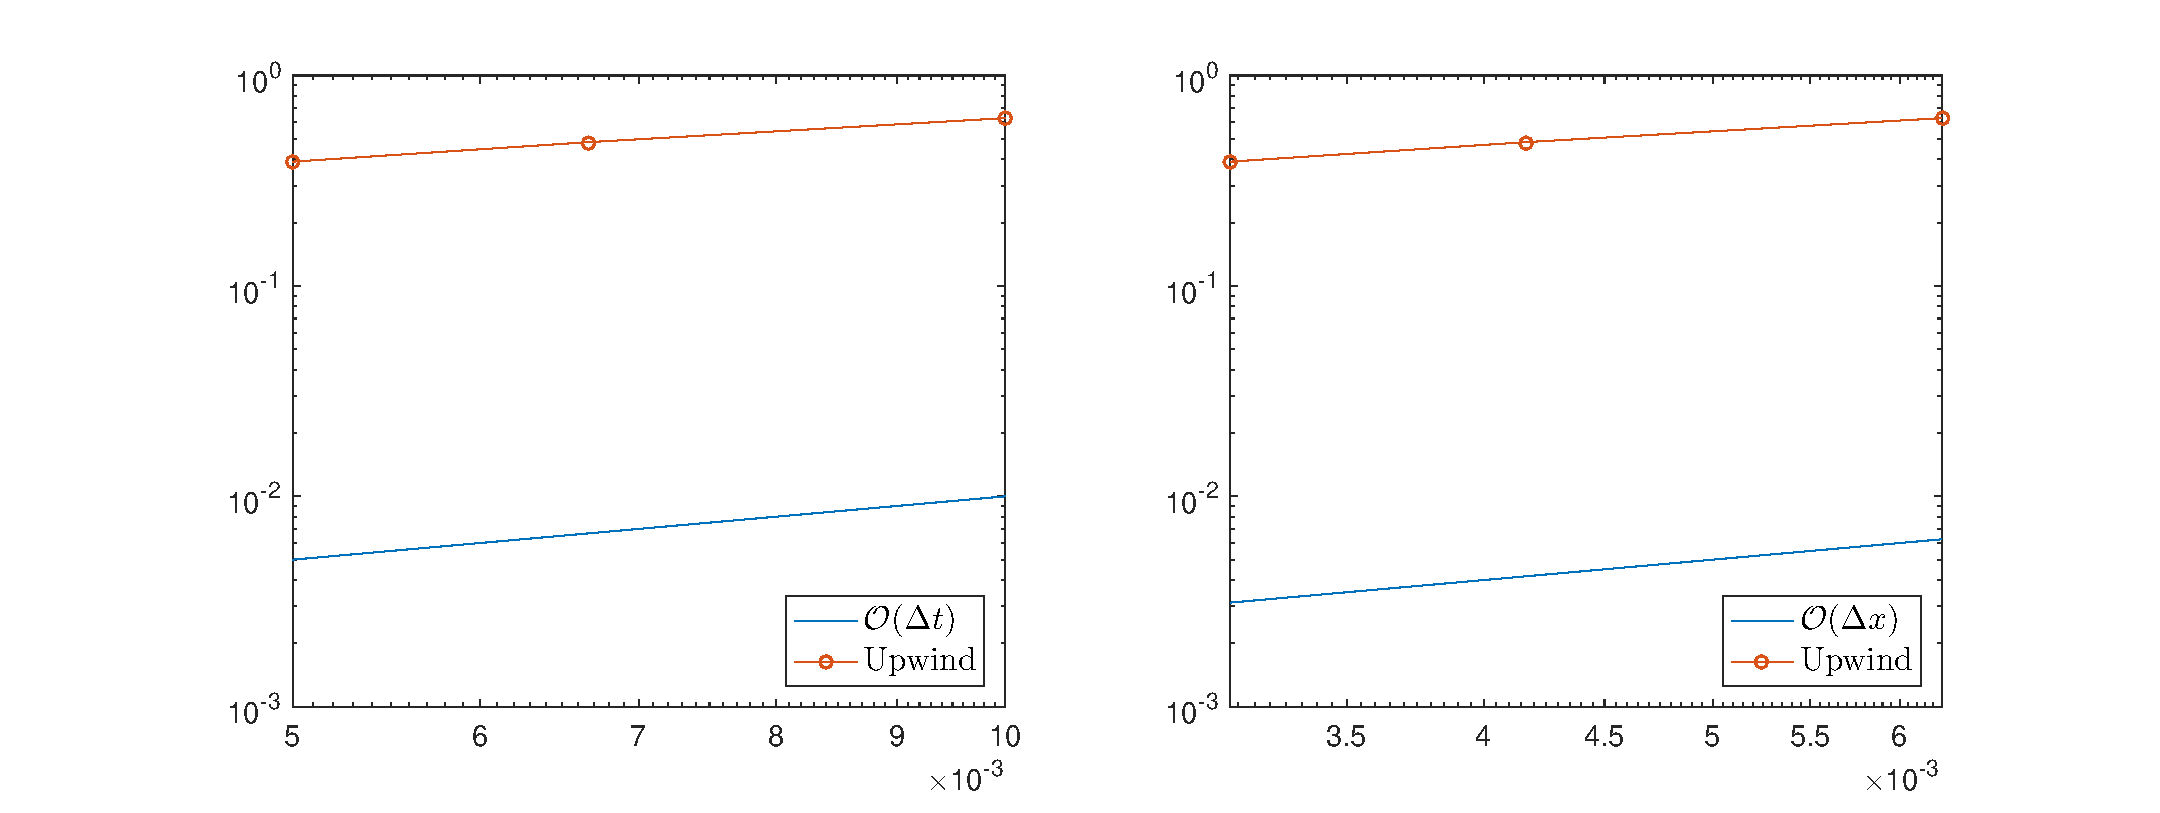
\includegraphics[width=\textwidth]{../Figures/ex2_2_convergence}
    \caption{Convergence of the Upwind method shown on the advection problem from 2.3, left plot is showcasing $\mathcal{O}(\Delta t)$ while the right one depicts $\mathcal{O}(\Delta x)$. Courant number was fixed at $\nu = 0.8$. The theoretical convergence is shown as a line and the calculated $\mathcal{O}$ as circles indicating the evaluated $\Delta t$ and $\Delta x$ in the logarithmic scale.}
\end{figure}

% 2.3
\subsection{Dispersion and diffusion}
Diffusion refers to the amplitude and dispersion to the phase, according to the slides from Lecture 23 the amplification factor $g(\xi)$ is used in the following way:
\begin{align}
    \mathrm{Diffusion} \quad & |g(\xi)| = \sqrt{ \left( 1 - \nu + \nu \cos(\phi) \right)^2 + \left( \nu \sin(\theta) \right)^2 } \\
    \mathrm{Dispersion} \quad & y = \tan^{-1}\frac{\Im(g(\xi))}{\Re(g(\xi))}
\end{align}
\subsubsection*{Predicting dispersion and diffusion}
Now the implementation of the upwind scheme will be tested and compared to the predicted dispersion and diffusion for the advection problem defined with the initial condition $u(x,t) = \sin(2 \pi x)$ on a periodic domain with Courant number $\nu = 0.8$ after 40 wave periods. The handout also says to use 100 points per one wave length in order to calculate the wave.

Going back to the equation \ref{ex2:eq:neumann} it is clear that the next time step is resolved as $g(\xi)^{n+1} = g(\xi)^n \left( 1 - \nu + \nu e^{-i \xi \Delta x} \right)$. For the given problem $\Delta x = \frac{1}{100}$, $\xi = 2 \pi$ and $\nu = \frac{8}{10}$. Using Matlab's \texttt{abs} and \texttt{angle} the following results are obtained:
\begin{align}
    |g(\xi)|^{\frac{T}{\Delta t}} &= |g(\xi)|^{\frac{80}{16/1000}} = |g(\xi)|^{5000} = 0.206157 \\
    \frac{y}{y_{\mathrm{true}}} &= \frac{\tan^{-1}\frac{\Im(g(\xi))}{\Re(g(\xi))}}{\nu \theta} =  1.000078971174729
\end{align}
Note that all the variables can be derived from the handout and using the definition of a sine wave moving to the right $y(x,t) = A \sin(kx - \omega t + \varphi) + D$, where $k = \frac{\omega}{v} = \frac{2 \pi f}{v} = \frac{2 \pi}{\lambda}$ ($v$ -- linear speed, $\lambda$ -- wave length). In this case $u$ can be written as $u(x,t) = 1 \sin(2 \pi x - \pi t + 0) + 0$ and $v = a = 0.5$. Having all the necessary information the Matlab implementation of the upwind scheme can be ran to $t_{\mathrm{max}} = 80$, with $\nu = 0.8$, $a = 0.5$, $\Delta x = 1/100$ and $\Delta t = 16/1000$.
\begin{figure}[h]
    \centering
    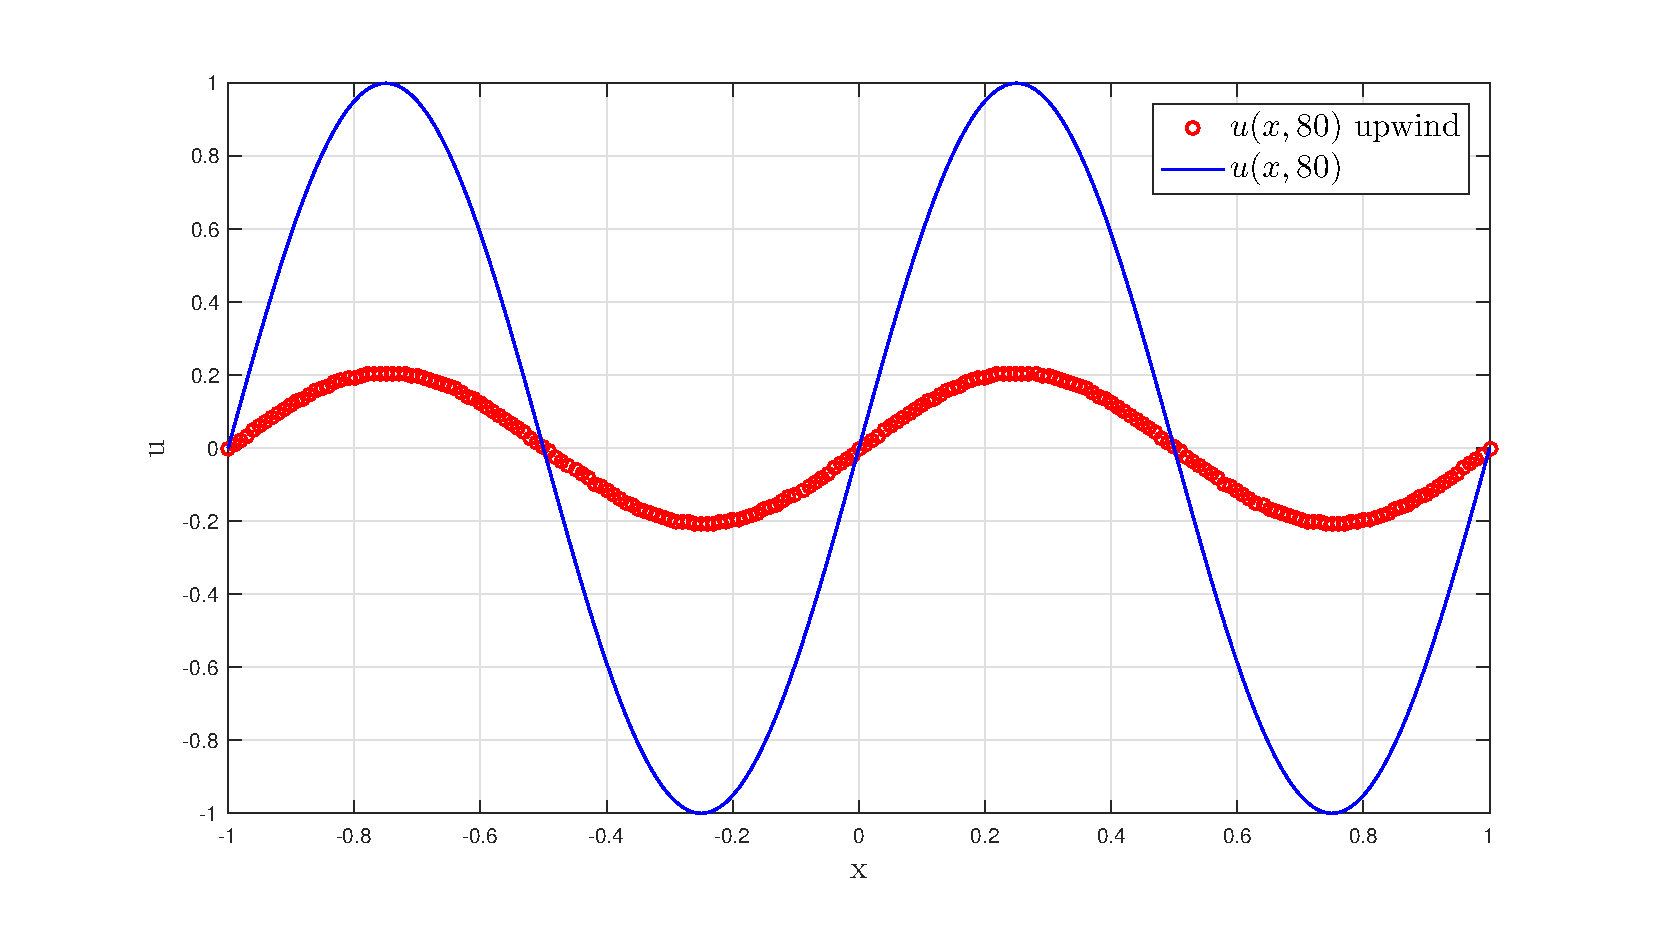
\includegraphics[width=\textwidth]{../Figures/ex2_3_upwind}
    \caption{Upwind scheme -- $x$ vs $u$ after 40 wave lengths for $\nu = 0.8$. The red points indicate the results from the implementation whereas the blue line is the true solution. Most notably the amplitude is damped to around 0.2 which corresponds to the theoretically obtained value.}
\end{figure}






















